\chapter{実験理論}\label{theory}



ポジトロニウムは陽電子と電子が電磁相互作用により束縛された系である.
陽電子は電子の反粒子で,電子と質量が等しく,電荷は逆で同じ大きさである.
後に詳しく述べるがポジトロニウムには,パラポジトロニウムとオルソポジトロニウムのふたつの状態があり,
量子電磁力学(QED)により寿命はそれぞれ125 ps,142 ns と計算されている.


\section{ポジトロニウムの状態}

電子のスピン演算子を
$\vector{\hat{S}}^{-} = (\hat{S}^{-}_{x},\hat{S}^{-}_{y},\hat{S}^{-}_{z})$
とする.
電子はスピン1/2なので,
$\hat{S}^{-^{2}}$
と
$\hat{S}^{-}_{z}$
の同時固有状態
\begin{equation}
\begin{split}
\hat{S}^{-^{2}} \ket{ \uparrow } = \frac{3}{4} \ket{ \uparrow },
\hat{S}^{-}_{z} \ket{ \uparrow } = + \frac{1}{2} \ket{ \uparrow } \\
\hat{S}^{-^{2}} \ket{ \downarrow } = \frac{3}{4} \ket{ \downarrow },
\hat{S}^{-}_{z} \ket{ \downarrow } = - \frac{1}{2} \ket{ \downarrow }
\end{split}
\label{eq:groundele}
\end{equation}
を基底にもつ.
電子の反粒子である陽電子についても同様に
\begin{equation}
\begin{split}
\hat{S}^{+^{2}} \ket{ \Uparrow } = \frac{3}{4} \ket{ \Uparrow },
\hat{S}^{+}_{z} \ket{ \Uparrow } = + \frac{1}{2} \ket{ \Uparrow } \\
\hat{S}^{+^{2}} \ket{ \Downarrow } = \frac{3}{4} \ket{ \Downarrow },
\hat{S}^{+}_{z} \ket{ \Downarrow } = - \frac{1}{2} \ket{ \Downarrow }
\end{split}
\label{eq:groundeposi}
\end{equation}
を基底にもつ.
以上のことからポジトロニウムの基底には
\begin{equation}
	\nonumber
\ket{ \uparrow } \ket{ \Uparrow },\ket{ \uparrow } \ket{ \Downarrow },
\ket{ \downarrow } \ket{ \Uparrow },\ket{ \downarrow } \ket{ \Downarrow }
\end{equation}
がとれる.
また系の全スピン $S = 0$ の1重項
\begin{equation}
\ket{0,0} = \frac{1}{\sqrt{2}} ( \ket{ \uparrow } \ket{ \Downarrow } - \ket{ \downarrow } \ket{ \Uparrow })
\label{eq:para}
\end{equation}
をパラポジトロニウム,
全スピン $S = 1$ の3重項
\begin{equation}
\begin{split}
&\ket{1,1} = \ket{ \uparrow } \ket{ \Uparrow } \\
&\ket{1,0} = \frac{1}{\sqrt{2}} ( \ket{ \uparrow } \ket{ \Downarrow } + \ket{ \downarrow } \ket{ \Uparrow }) \\
&\ket{1,-1} = \ket{ \downarrow } \ket{ \Downarrow }
\end{split}
\label{eq:ortho}
\end{equation}
をオルソポジトロニウムと呼ぶ.(図\ref{fig:Ps})

\begin{figure}[H]
\centering
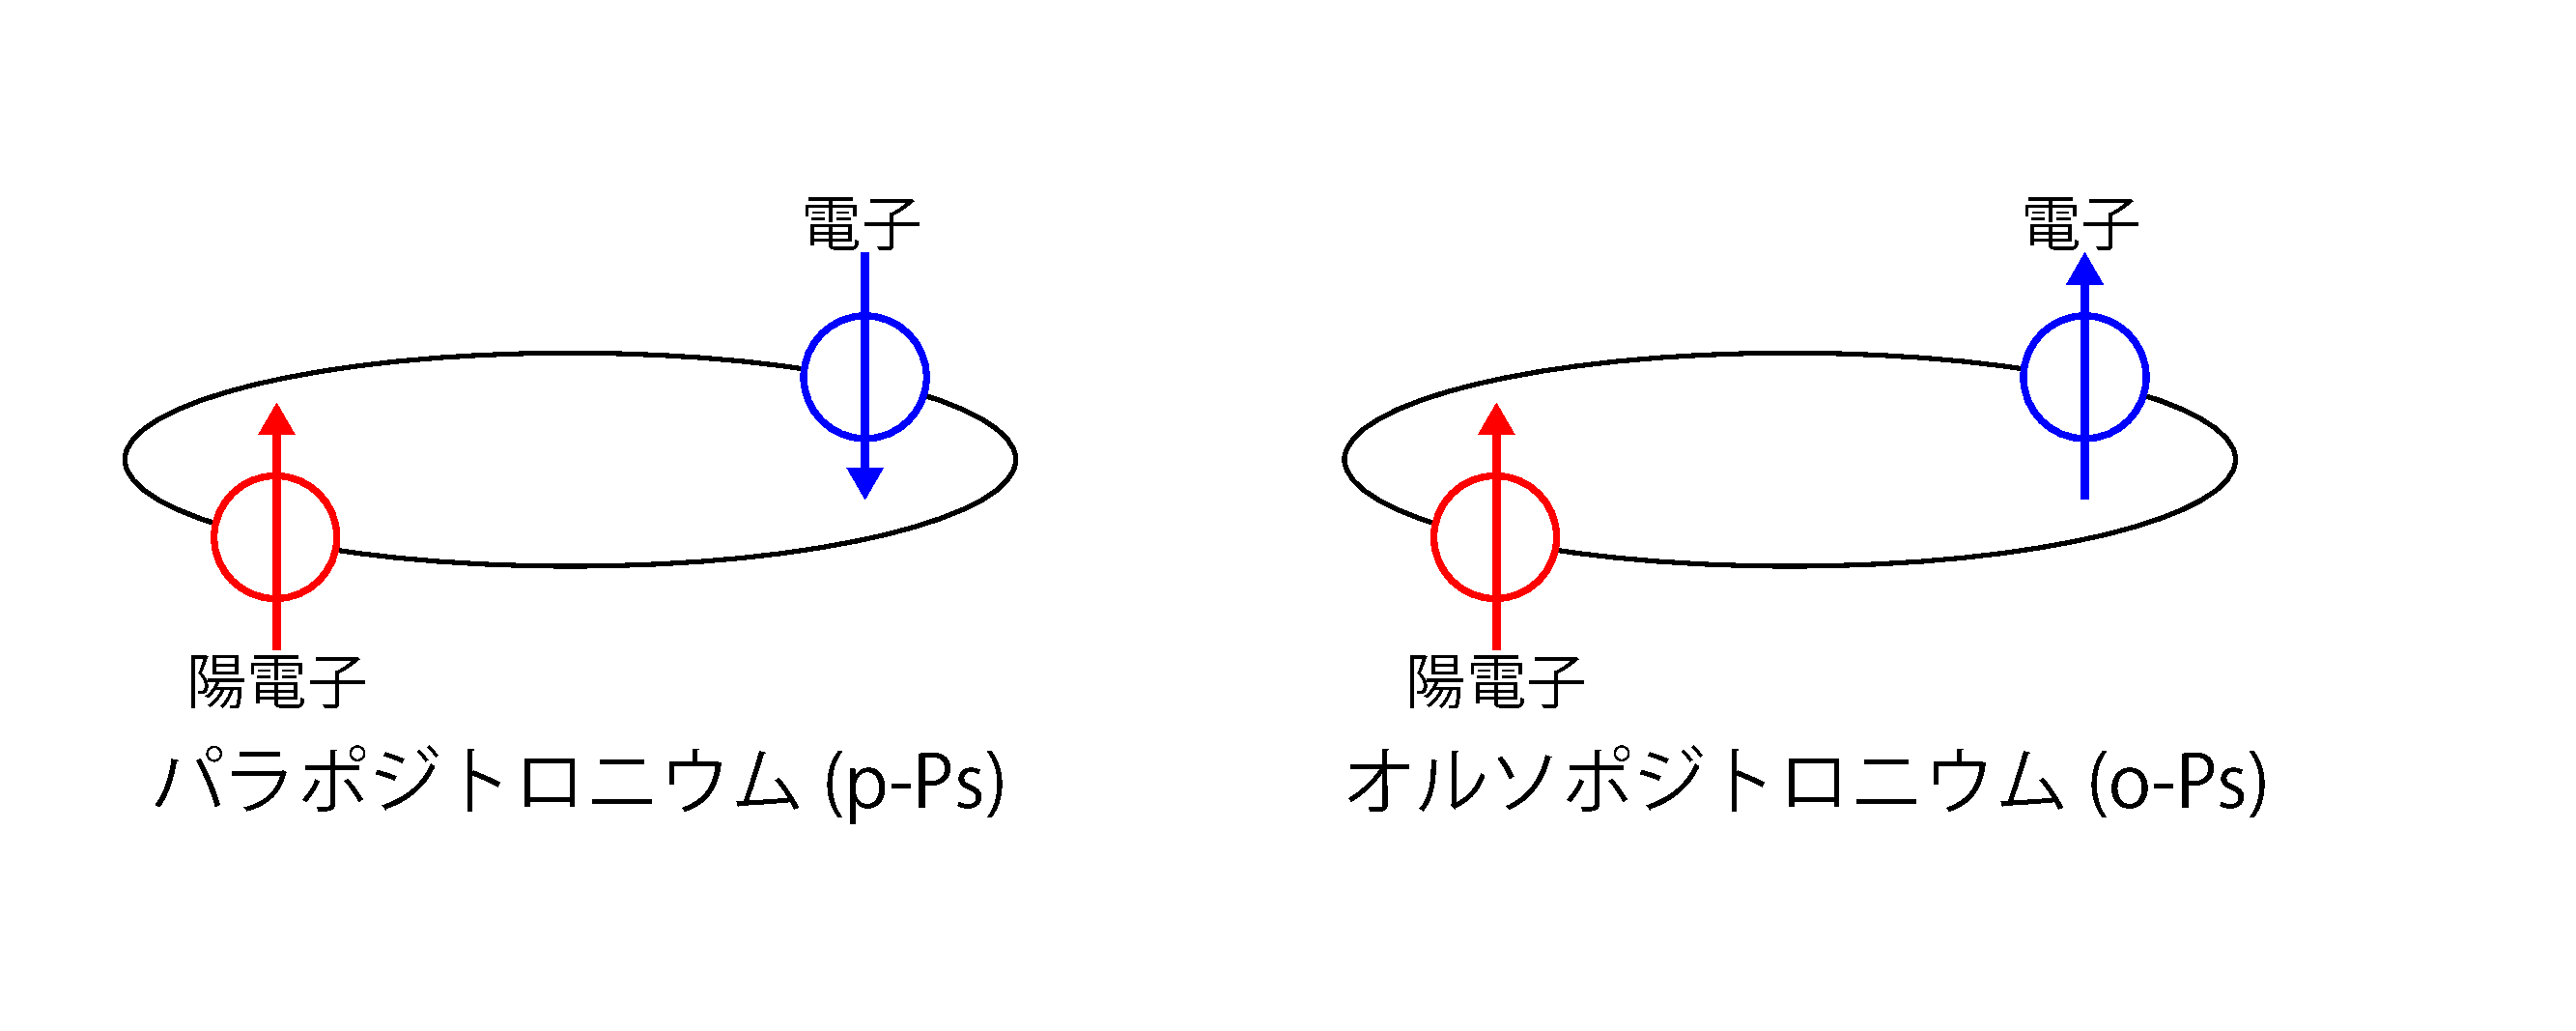
\includegraphics[keepaspectratio, scale=0.4]{fig/ybm/Ps.pdf}
\caption{ポジトロニウムのふたつの状態}
\label{fig:Ps}
\end{figure}


\section{ポジトロニウムの崩壊}

ポジトロニウムはいくつかの光子に崩壊する.
パラポジトロニウムの全スピンは $S=0$ であるので,
基底状態のCパリティは

\begin{equation}
	\nonumber
C = (-1)^{S} = 1
\end{equation}
となり,オルソポジトロニウムの全スピンは $S=1$ であるので,
基底状態のCパリティは
\begin{equation}
	\nonumber
C = (-1)^{S} = -1
\end{equation}
となる.
ここで$n$個の光子のCパリティは
\begin{equation}
	\nonumber
C = (-1)^{n}
\end{equation}
であるので,
Cパリティの保存より,
パラポジトロニウムは偶数本,オルソポジトロニウムは奇数本の光子へのみ崩壊する.
ポジトロニウムの崩壊率は,
放出される光子の数が1つ増えるごとに微細構造定数 $\alpha \sim 1/137$ の因子がかかり小さくなるので,
運動量保存を考えると,
パラポジトロニウムは2光子崩壊,オルソポジトロニウムは3光子崩壊が支配的であることがわかる.
エネルギー保存より,ガンマ線のエネルギーはパラポジトロニウムが 511 keV,
オルソポジトロニウムが $0 \sim 511$  keVの連続スペクトルとなる.

また量子電磁力学により寿命はパラポジトロニウムが
\begin{equation}
	\nonumber
\tau_{p} = \frac{m \alpha^{5}}{2} \simeq 125 \, \si{ps}
\end{equation}
オルソポジトロニウムが
\begin{equation}
	\nonumber
\tau_{o} = \frac{2m \alpha^{6}(\pi^{2}-9)}{9 \pi} \simeq 142 \, \si{ns}
\end{equation}
と計算されている.


\section{ポジトロニウムの超微細構造}

パラポジトロニウムとオルソポジトロニウムは,
それぞれのスピン同士の相互作用によりエネルギー準位がずれている.
このずれを超微細構造と呼び,その値は
\begin{equation}
	\nonumber
\Delta_{\mathrm{HFS}} \simeq 0.84 \, \mathrm{meV}
\end{equation}
と計算されている.


\section{磁場中のポジトロニウム}
ポジトロニウムに磁場を印加すると,ポジトロニウムの基底状態が混合する.
まず磁場を$z$方向にとり,大きさを$B$とすると,
磁場によるハミルトニアンは
\begin{equation}
	\nonumber
	\hat{H}_{B} = g\mu_{\mathrm{B}}B(\hat{S}^{-}_{z} - \hat{S}^{+}_{z})
\end{equation}
となる.
$g$はLandeの$g$因子,$\mu_{\mathrm{B}}$はボーア磁子である.%\noindent
(\ref{eq:groundele})(\ref{eq:groundeposi})(\ref{eq:para})(\ref{eq:ortho})より
\begin{align}
	\nonumber
(\hat{S}^{-}_{z} - \hat{S}^{+}_{z})\ket{0,0} &= (\hat{S}^{-}_{z} - \hat{S}^{+}_{z})\frac{1}{\sqrt{2}} ( \ket{ \uparrow } \ket{ \Downarrow } - \ket{ \downarrow } \ket{ \Uparrow }) \notag \\
&= \frac{1}{2\sqrt{2}} ( \ket{ \uparrow } \ket{ \Downarrow } + \ket{ \downarrow } \ket{ \Uparrow } - ( - \ket{ \uparrow } \ket{ \Downarrow } - \ket{ \downarrow } \ket{ \Uparrow } )) \notag \\
&= \frac{1}{\sqrt{2}} ( \ket{ \uparrow } \ket{ \Downarrow } + \ket{ \downarrow } \ket{ \Uparrow }) = \ket{1,0} \\
(\hat{S}^{-}_{z} - \hat{S}^{+}_{z})\ket{1,1}
&= (\hat{S}^{-}_{z} - \hat{S}^{+}_{z})\ket{ \uparrow } \ket{ \Uparrow }
=\frac{1}{2}( \ket{ \uparrow } \ket{ \Uparrow } - \ket{ \uparrow } \ket{ \Uparrow } )
= 0 \\
(\hat{S}^{-}_{z} - \hat{S}^{+}_{z})\ket{1,0} &= (\hat{S}^{-}_{z} - \hat{S}^{+}_{z})\frac{1}{\sqrt{2}} ( \ket{ \uparrow } \ket{ \Downarrow } + \ket{ \downarrow } \ket{ \Uparrow }) \notag \\
&= \frac{1}{2\sqrt{2}} ( \ket{ \uparrow } \ket{ \Downarrow } - \ket{ \downarrow } \ket{ \Uparrow } - ( - \ket{ \uparrow } \ket{ \Downarrow } + \ket{ \downarrow } \ket{ \Uparrow } )) \notag \\
&= \frac{1}{\sqrt{2}} ( \ket{ \uparrow } \ket{ \Downarrow } - \ket{ \downarrow } \ket{ \Uparrow }) = \ket{0,0} \\
(\hat{S}^{-}_{z} - \hat{S}^{+}_{z})\ket{1,-1}
&= (\hat{S}^{-}_{z} - \hat{S}^{+}_{z})\ket{ \downarrow } \ket{ \Downarrow }
=\frac{1}{2}( - \ket{ \downarrow } \ket{ \Downarrow } + \ket{ \downarrow } \ket{ \Downarrow } )
= 0
\end{align}
となり,$\ket{0,0}$と$\ket{1,0}$の状態が磁場によって混合し,
新たなエネルギー固有状態$\ket{+}$,$\ket{-}$がつくられる.
ここで以下で用いるパラメータ
\begin{equation}
	\nonumber
	x = \frac{2g\mu_{\mathrm{B}}B}{\Delta_{\mathrm{HFS}}}
\end{equation}
を導入する.
$\ket{+}$に占める$\ket{0,0}$の割合は
\begin{equation}
	\nonumber
\frac{ \frac{x^{2}}{4} \left(1-\frac{x^{2}}{4}\right)^{2}  }{  1+\frac{x^{2}}{4}\left( 1-\frac{x^{2}}{4} \right)^2   }
\end{equation}
となる.(図\ref{fig:plusstate})
また$\ket{-}$に占める$\ket{0,0}$の割合は
\begin{equation}
	\nonumber
\frac{1}{1+\frac{x^{2}}{4}\left(1-\frac{x^{2}}{4}\right)^{2}}
\end{equation}
となる.(図\ref{fig:minusstate})

\begin{figure}[H]
\centering
\includegraphics[keepaspectratio,angle=270,scale=0.6]{fig/ybm/plusstate.pdf}
\caption{$\ket{+}$に占める$\ket{0,0}$の割合}
\label{fig:plusstate}
\end{figure}

\begin{figure}[H]
\centering
\includegraphics[keepaspectratio,angle=270,scale=0.6]{fig/ybm/minusstate.pdf}
\caption{$\ket{-}$に占める$\ket{0,0}$の割合}
\label{fig:minusstate}
\end{figure}

また$\ket{+}$の寿命は
\begin{equation}
	\nonumber
\frac{4}{\frac{1}{\tau_{p}}x^{2}+\frac{1}{\tau_{o}(4-x^{2})}}
\end{equation}
となり,(図\ref{fig:pluslife})
$\ket{-}$の寿命は
\begin{equation}
	\nonumber
\frac{4}{\frac{1}{\tau_{p}(4-x^{2})}+\frac{1}{\tau_{o}}x^{2}}
\end{equation}
となる.(図\ref{fig:minuslife})

\begin{figure}[H]
\centering
\includegraphics[keepaspectratio,angle=270,scale=0.6]{fig/ybm/pluslife.pdf}
\caption{$\ket{+}$の寿命}
\label{fig:pluslife}
\end{figure}

\begin{figure}[H]
\centering
\includegraphics[keepaspectratio,angle=270,scale=0.6]{fig/ybm/minuslife.pdf}
\caption{$\ket{-}$の寿命}
\label{fig:minuslife}
\end{figure}


\section{物質中でのポジトロニウム}

物質中ではポジトロニウム中の電子と陽電子の対消滅以外の要因で崩壊し,
通常よりも寿命が短くなる.
この要因としては次の3つがある.
\begin{itemize}
\item Pick off:ポジトロニウム中の陽電子が,物質中の電子と対消滅する.
\item Spin flip:オルソポジトロニウム中の電子が,物質中の不対電子とスピンを交換しパラポジトロニウムとなる.
\item 化学反応:酸化反応によりポジトロニウムから電子が奪われ,自由になった陽電子が物質中の電子と対消滅する.
\end{itemize}
これらは密度の低いシリカエアロゲルを用い,
また空気中の水分子の影響を小さくするためにシリカエアロゲルを熱することで抑えられる.


\begin{comment}
\section{プラスチックシンチレータ}

ポジトロニウムを形成するための陽電子源に使用している$\mathrm{^{22}Na}$は,
$\beta^{+}$崩壊(式\ref{eq:beta},図\ref{fig:na})をする.
\begin{equation}
\mathrm{^{22}Na} \to \mathrm{^{22}Ne} + \mathrm{e^{+}} + \nu_{\mathrm{e}}
\label{eq:beta}
\end{equation}

\begin{figure}[H]
\centering
\includegraphics[keepaspectratio,scale=0.4]{fig/ybm/na.pdf}
\caption{$\mathrm{^{22}Na}$の崩壊}
\label{fig:na}
\end{figure}

昨年度まではトリガーに1.275 MeVの$\gamma$線を使用していたが,

\end{comment}

%\end{document}
